% Created by tikzDevice version 0.12.6 on 2024-08-01 12:50:02
% !TEX encoding = UTF-8 Unicode
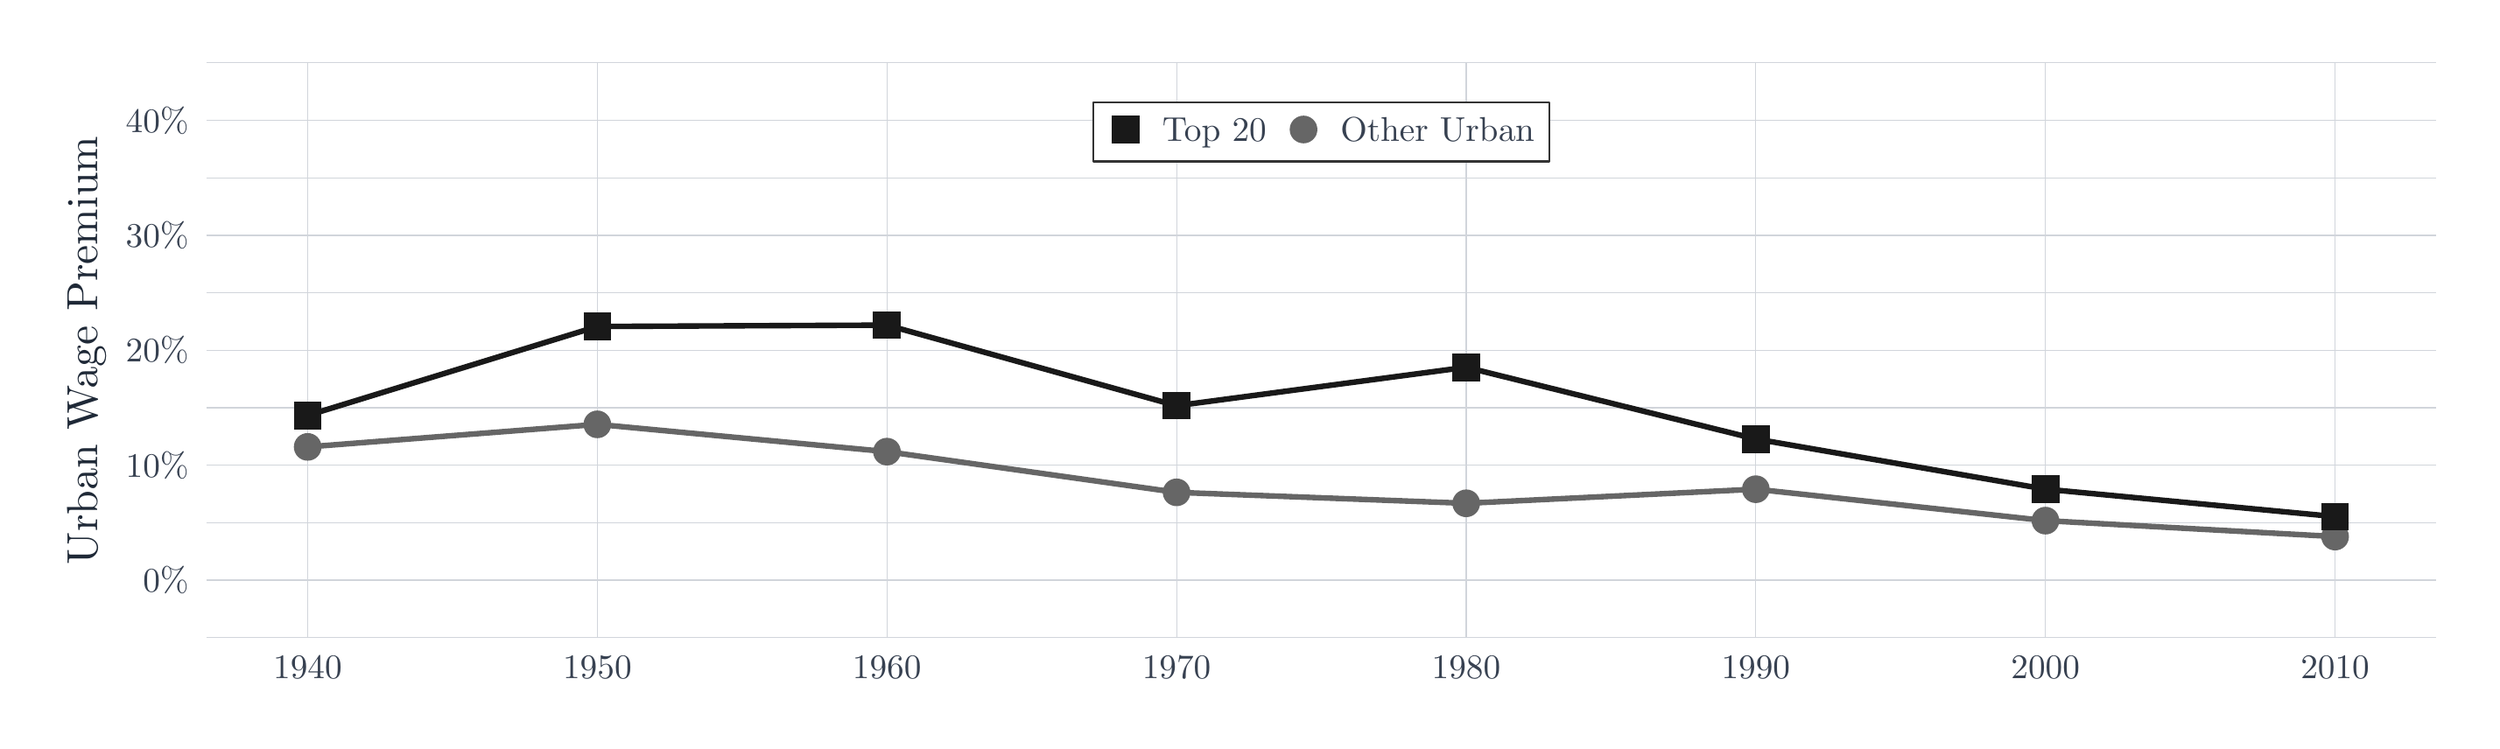
\begin{tikzpicture}[x=1pt,y=1pt]
\definecolor{fillColor}{RGB}{255,255,255}
\path[use as bounding box,fill=fillColor] (0,0) rectangle (1011.78,289.08);
\begin{scope}
\path[clip] (  0.00,  0.00) rectangle (1011.78,289.08);
\definecolor{drawColor}{RGB}{255,255,255}

\path[draw=drawColor,line width= 0.8pt,line join=round,line cap=round,fill=fillColor] (  0.00,  0.00) rectangle (1011.78,289.08);
\end{scope}
\begin{scope}
\path[clip] ( 75.16, 35.76) rectangle (995.78,273.08);
\definecolor{drawColor}{RGB}{255,255,255}
\definecolor{fillColor}{RGB}{255,255,255}

\path[draw=drawColor,line width= 0.8pt,line join=round,line cap=round,fill=fillColor] ( 75.16, 35.76) rectangle (995.78,273.08);
\definecolor{drawColor}{RGB}{209,213,219}

\path[draw=drawColor,line width= 0.4pt,line join=round] ( 75.16, 35.76) --
	(995.78, 35.76);

\path[draw=drawColor,line width= 0.4pt,line join=round] ( 75.16, 83.22) --
	(995.78, 83.22);

\path[draw=drawColor,line width= 0.4pt,line join=round] ( 75.16,130.69) --
	(995.78,130.69);

\path[draw=drawColor,line width= 0.4pt,line join=round] ( 75.16,178.15) --
	(995.78,178.15);

\path[draw=drawColor,line width= 0.4pt,line join=round] ( 75.16,225.62) --
	(995.78,225.62);

\path[draw=drawColor,line width= 0.4pt,line join=round] ( 75.16,273.08) --
	(995.78,273.08);

\path[draw=drawColor,line width= 0.4pt,line join=round] ( 75.16, 59.49) --
	(995.78, 59.49);

\path[draw=drawColor,line width= 0.4pt,line join=round] ( 75.16,106.95) --
	(995.78,106.95);

\path[draw=drawColor,line width= 0.4pt,line join=round] ( 75.16,154.42) --
	(995.78,154.42);

\path[draw=drawColor,line width= 0.4pt,line join=round] ( 75.16,201.88) --
	(995.78,201.88);

\path[draw=drawColor,line width= 0.4pt,line join=round] ( 75.16,249.35) --
	(995.78,249.35);

\path[draw=drawColor,line width= 0.4pt,line join=round] (117.01, 35.76) --
	(117.01,273.08);

\path[draw=drawColor,line width= 0.4pt,line join=round] (236.57, 35.76) --
	(236.57,273.08);

\path[draw=drawColor,line width= 0.4pt,line join=round] (356.13, 35.76) --
	(356.13,273.08);

\path[draw=drawColor,line width= 0.4pt,line join=round] (475.69, 35.76) --
	(475.69,273.08);

\path[draw=drawColor,line width= 0.4pt,line join=round] (595.25, 35.76) --
	(595.25,273.08);

\path[draw=drawColor,line width= 0.4pt,line join=round] (714.81, 35.76) --
	(714.81,273.08);

\path[draw=drawColor,line width= 0.4pt,line join=round] (834.37, 35.76) --
	(834.37,273.08);

\path[draw=drawColor,line width= 0.4pt,line join=round] (953.93, 35.76) --
	(953.93,273.08);
\definecolor{drawColor}{gray}{0.10}

\path[draw=drawColor,line width= 2.3pt,line join=round] (117.01,127.51) --
	(236.57,164.25) --
	(356.13,164.82) --
	(475.69,131.53) --
	(595.25,147.40) --
	(714.81,117.78) --
	(834.37, 97.07) --
	(953.93, 85.74);
\definecolor{drawColor}{gray}{0.40}

\path[draw=drawColor,line width= 2.3pt,line join=round] (117.01,114.52) --
	(236.57,123.83) --
	(356.13,112.56) --
	(475.69, 95.75) --
	(595.25, 91.23) --
	(714.81, 97.05) --
	(834.37, 84.07) --
	(953.93, 77.49);
\definecolor{fillColor}{gray}{0.40}

\path[fill=fillColor] (117.01,114.52) circle (  5.71);
\definecolor{fillColor}{gray}{0.10}

\path[fill=fillColor] (111.30,121.80) --
	(122.72,121.80) --
	(122.72,133.22) --
	(111.30,133.22) --
	cycle;
\definecolor{fillColor}{gray}{0.40}

\path[fill=fillColor] (236.57,123.83) circle (  5.71);
\definecolor{fillColor}{gray}{0.10}

\path[fill=fillColor] (230.86,158.54) --
	(242.28,158.54) --
	(242.28,169.96) --
	(230.86,169.96) --
	cycle;
\definecolor{fillColor}{gray}{0.40}

\path[fill=fillColor] (356.13,112.56) circle (  5.71);
\definecolor{fillColor}{gray}{0.10}

\path[fill=fillColor] (350.42,159.11) --
	(361.84,159.11) --
	(361.84,170.53) --
	(350.42,170.53) --
	cycle;
\definecolor{fillColor}{gray}{0.40}

\path[fill=fillColor] (475.69, 95.75) circle (  5.71);
\definecolor{fillColor}{gray}{0.10}

\path[fill=fillColor] (469.98,125.82) --
	(481.40,125.82) --
	(481.40,137.24) --
	(469.98,137.24) --
	cycle;
\definecolor{fillColor}{gray}{0.40}

\path[fill=fillColor] (595.25, 91.23) circle (  5.71);
\definecolor{fillColor}{gray}{0.10}

\path[fill=fillColor] (589.54,141.69) --
	(600.96,141.69) --
	(600.96,153.12) --
	(589.54,153.12) --
	cycle;
\definecolor{fillColor}{gray}{0.40}

\path[fill=fillColor] (714.81, 97.05) circle (  5.71);
\definecolor{fillColor}{gray}{0.10}

\path[fill=fillColor] (709.10,112.07) --
	(720.52,112.07) --
	(720.52,123.49) --
	(709.10,123.49) --
	cycle;
\definecolor{fillColor}{gray}{0.40}

\path[fill=fillColor] (834.37, 84.07) circle (  5.71);
\definecolor{fillColor}{gray}{0.10}

\path[fill=fillColor] (828.66, 91.36) --
	(840.08, 91.36) --
	(840.08,102.79) --
	(828.66,102.79) --
	cycle;
\definecolor{fillColor}{gray}{0.40}

\path[fill=fillColor] (953.93, 77.49) circle (  5.71);
\definecolor{fillColor}{gray}{0.10}

\path[fill=fillColor] (948.22, 80.03) --
	(959.64, 80.03) --
	(959.64, 91.45) --
	(948.22, 91.45) --
	cycle;
\end{scope}
\begin{scope}
\path[clip] (  0.00,  0.00) rectangle (1011.78,289.08);
\definecolor{drawColor}{RGB}{55,65,81}

\node[text=drawColor,anchor=base east,inner sep=0pt, outer sep=0pt, scale=  1.42] at ( 67.96, 54.59) {0\%};

\node[text=drawColor,anchor=base east,inner sep=0pt, outer sep=0pt, scale=  1.42] at ( 67.96,102.06) {10\%};

\node[text=drawColor,anchor=base east,inner sep=0pt, outer sep=0pt, scale=  1.42] at ( 67.96,149.52) {20\%};

\node[text=drawColor,anchor=base east,inner sep=0pt, outer sep=0pt, scale=  1.42] at ( 67.96,196.99) {30\%};

\node[text=drawColor,anchor=base east,inner sep=0pt, outer sep=0pt, scale=  1.42] at ( 67.96,244.45) {40\%};
\end{scope}
\begin{scope}
\path[clip] (  0.00,  0.00) rectangle (1011.78,289.08);
\definecolor{drawColor}{RGB}{55,65,81}

\node[text=drawColor,anchor=base,inner sep=0pt, outer sep=0pt, scale=  1.42] at (117.01, 18.76) {1940};

\node[text=drawColor,anchor=base,inner sep=0pt, outer sep=0pt, scale=  1.42] at (236.57, 18.76) {1950};

\node[text=drawColor,anchor=base,inner sep=0pt, outer sep=0pt, scale=  1.42] at (356.13, 18.76) {1960};

\node[text=drawColor,anchor=base,inner sep=0pt, outer sep=0pt, scale=  1.42] at (475.69, 18.76) {1970};

\node[text=drawColor,anchor=base,inner sep=0pt, outer sep=0pt, scale=  1.42] at (595.25, 18.76) {1980};

\node[text=drawColor,anchor=base,inner sep=0pt, outer sep=0pt, scale=  1.42] at (714.81, 18.76) {1990};

\node[text=drawColor,anchor=base,inner sep=0pt, outer sep=0pt, scale=  1.42] at (834.37, 18.76) {2000};

\node[text=drawColor,anchor=base,inner sep=0pt, outer sep=0pt, scale=  1.42] at (953.93, 18.76) {2010};
\end{scope}
\begin{scope}
\path[clip] (  0.00,  0.00) rectangle (1011.78,289.08);
\definecolor{drawColor}{RGB}{31,41,55}

\node[text=drawColor,rotate= 90.00,anchor=base,inner sep=0pt, outer sep=0pt, scale=  1.80] at ( 30.15,154.42) {Urban Wage Premium};
\end{scope}
\begin{scope}
\path[clip] (  0.00,  0.00) rectangle (1011.78,289.08);
\definecolor{drawColor}{gray}{0.20}
\definecolor{fillColor}{RGB}{255,255,255}

\path[draw=drawColor,line width= 0.8pt,line join=round,line cap=round,fill=fillColor] (441.37,232.37) rectangle (629.57,256.83);
\end{scope}
\begin{scope}
\path[clip] (  0.00,  0.00) rectangle (1011.78,289.08);
\definecolor{drawColor}{RGB}{255,255,255}
\definecolor{fillColor}{RGB}{255,255,255}

\path[draw=drawColor,line width= 0.8pt,line join=round,line cap=round,fill=fillColor] (447.37,238.37) rectangle (461.83,252.83);
\end{scope}
\begin{scope}
\path[clip] (  0.00,  0.00) rectangle (1011.78,289.08);
\definecolor{fillColor}{gray}{0.10}

\path[fill=fillColor] (448.89,239.89) --
	(460.31,239.89) --
	(460.31,251.31) --
	(448.89,251.31) --
	cycle;
\end{scope}
\begin{scope}
\path[clip] (  0.00,  0.00) rectangle (1011.78,289.08);
\definecolor{drawColor}{RGB}{255,255,255}
\definecolor{fillColor}{RGB}{255,255,255}

\path[draw=drawColor,line width= 0.8pt,line join=round,line cap=round,fill=fillColor] (520.87,238.37) rectangle (535.32,252.83);
\end{scope}
\begin{scope}
\path[clip] (  0.00,  0.00) rectangle (1011.78,289.08);
\definecolor{fillColor}{gray}{0.40}

\path[fill=fillColor] (528.10,245.60) circle (  5.71);
\end{scope}
\begin{scope}
\path[clip] (  0.00,  0.00) rectangle (1011.78,289.08);
\definecolor{drawColor}{RGB}{55,65,81}

\node[text=drawColor,anchor=base west,inner sep=0pt, outer sep=0pt, scale=  1.42] at (469.83,240.70) {Top 20};
\end{scope}
\begin{scope}
\path[clip] (  0.00,  0.00) rectangle (1011.78,289.08);
\definecolor{drawColor}{RGB}{55,65,81}

\node[text=drawColor,anchor=base west,inner sep=0pt, outer sep=0pt, scale=  1.42] at (543.32,240.70) {Other Urban};
\end{scope}
\end{tikzpicture}
